\scanpage{52}
\uline{Lemme} Soient $K$ un corps, $G$ un groupe algébrique sur $K$, $M=(M(n))$ un groupe p-divisible ($p$ un nb premier), \deleted{a) Si $\operatorname{car}K=p$,} $\varphi:M\mathbin{-}G$ un hom de groupes. ! Alors \inserted{\figure{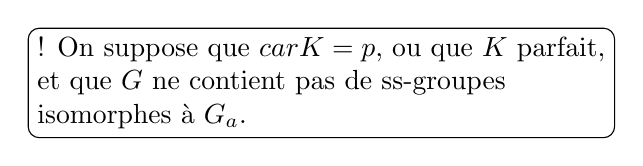
\begin{tikzpicture}\node[draw,rounded corners,align=left] {! On suppose que $\operatorname{car}K=p$, ou \unsure{que} $K$ parfait,\\et que $G$ ne contient pas de ss-groupes\\isomorphes à $G_a$.};\end{tikzpicture}}} il existe un sous-schéma en groupes $H$ de $G$, extension d'une VA par un tore, tel que $\varphi$ se factorise par $H$.
\deleted{b) Si $\operatorname{car}K=$}

\uline{Dém} On a $\varphi=(\varphi(n))$, avec
\[
\varphi(n):M(n)\longrightarrow G
\]
Soit $Z_n=\operatorname{Cent}\varphi(n)$. Les $Z_n$ sont des sous-schémas en groupes fermés en suite décroissante, donc stationnaire, soit $Z$ la valeur commune.

Evidemment $\varphi$ se factorise par \deleted{$\unsure{G}$} $Z$, et même par $\operatorname{Cent}(Z)$. Cela nous ramène au cas où $G$ est commutatif. Evidemment \deleted{on} \inserted{l'hom} composé $M\mathbin{-}G\mathbin{-}G/G^0$ est nul, donc on peut supposer $G$ connexe.

\uline{1º Cas} $p=\operatorname{car}K$. On a évidemment, pour $\forall$ entier $\nu\geq0$, que $\varphi$ se factorise par $p^\nu G$. Or pour $\nu$ grand, on sait \deleted{$\unsure{p^\nu G}$} que $p^\nu G$ est une extension d'une VA par un tore (à dégager un lemme, vrai $\forall$ groupe algébrique commutatif sur un corps de car. $p>0$).

\uline{2ème Cas} \deleted{$\unsure{p\ne\operatorname{car}K}$. Les $M(n)$ sont tous étales.} \inserted{\deleted{\unsure{car}} $K$ parfait, $G$ n'a pas de ss-groupe isom : $G_a$.}
Alors on sait que $G$ est ext d'une VA. par un tore!

\mspage{51}
